\documentclass[twoside,letterpaper]{refrep}
\usepackage{makeidx}
\usepackage{natbib}
\usepackage{xspace}
\usepackage{graphicx}
\usepackage{verbatim}
\usepackage{threeparttable}

\settextfraction{1.0}

\newcommand{\facversion}{{0.7.2}\xspace}

\newenvironment{mydesc}{\textbf{Field Description:} \begin{list}
	{:}{\setlength{\labelwidth}{2in}
	   \setlength{\leftmargin}{2in}
	   \setlength{\labelsep}{0.1in}
	   \setlength{\rightmargin}{0.2in}}}
	{\end{list}}

\setcounter{tocdepth}{2}

\makeindex

\begin{document}

\title{FAC \facversion Manual}
\author{M. F. Gu\thanks{Chandra Fellow,  mfgu@space.mit.edu} \\
Center for Space Research, MIT \\ Cambridge, MA 02139}

\date{}

\maketitle

\tableofcontents

\chapter{Overview}
\label{cha:overview}

\section{What Is FAC}
FAC stands for The Flexible Atomic Code (and nothing else). It is an
integrated software package to calculate various atomic radiative and
collisional processes, including energy levels, radiative transition rates,
collisional excitation and 
ionization by electron impact, photoionization, autoionization, radiative
recombination and dielectronic capture. The package also includes a
collisional radiative model to construct synthetic spectra for plasmas under
different physical conditions. The various parts of FAC and their
interactions are shown in Figure \ref{fig:flow}. 

\begin{figure}
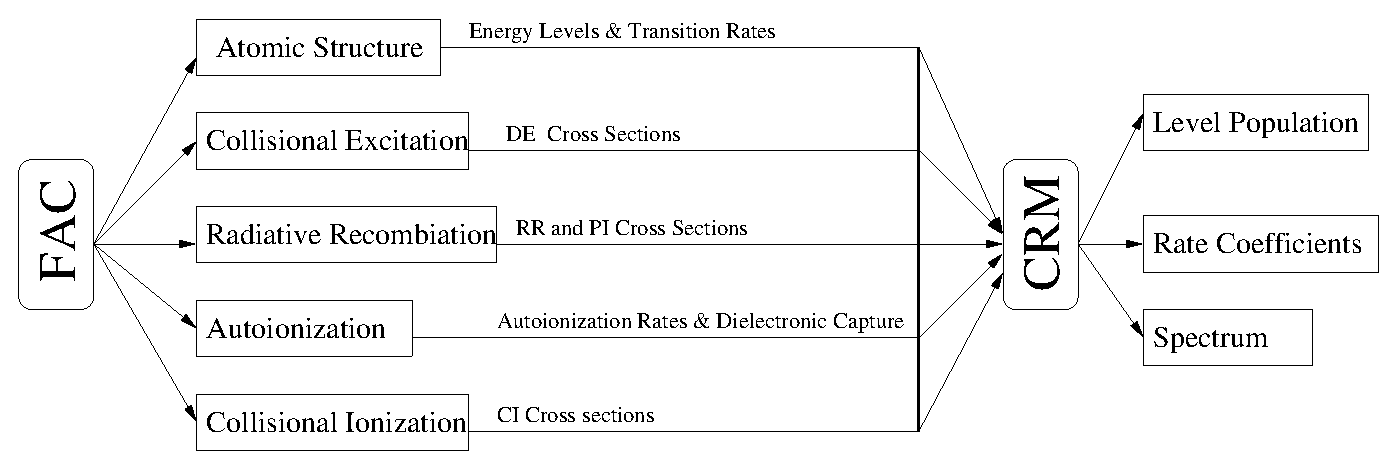
\includegraphics[width=6in]{flow.eps}
\caption{\label{fig:flow}The overview of FAC package.}
\end{figure}

The atomic structure calculation in FAC is based on the relativistic
configuration interaction with independent particle basis wavefunctions. These
basis wavefunctions are derived from a local central potential, which is
self-consistently determined to represent electronic screening of the nuclear
potential. Relativistic effects are fully taken into account using the Dirac
Coulomb Hamiltonian. Higher order QED effects are presently ignored, which may
limit its accuracy for very high-$Z$ elements. Continuum processes are treated
in the distorted-wave (DW) approximation. Systematic application of the
factorization-interpolation method of \citet{barshalom88} makes the present
code highly efficient for large scale calculations. The details of theoretical
background and computational methods are not discussed in this manual, in
stead, they are described in a series of papers which are distributed along
with this package and this manual.

FAC is a step forward to bring detailed atomic model accessable to a wide
community of laboratory and astrophysical plasma diagnostics. Its flexible
interface is designed to be useful even for people without a deep
understanding of the underlying atomic theories. It is also powerful enough
for experieced users to explore the effects of algorithmic choices and
different physical approximations.

FAC is freely distributed in the hope that it will be useful. The author makes
every effort to ensure its correctness. However, he does not guarantee its
fitness to any specific purpose. The author is not responsible for any damage
resulting from the use of this program, including failure to obtain or loss of
tenure. 

\section{Obtain and Install FAC}
\index{Install}
\label{sec:install}
The latest version of FAC is \facversion. It can be obtained from anounymous
ftp://space.mit.edu/pub/mfgu/fac/. I can also send a copy to you through
email. Please request to \textbf{mfgu@space.mit.edu}. It is being continously
developed at present, so please check regularly to get the newest version. 

Much of the FAC package is written in ANSI C and Fortran 77. It should 
therefore work on any platform with a C and Fortran 77 compilers. However, 
this is only true to the rather simple command parser come with FAC, referred 
to as SFAC. The flexibility of FAC is realized when the Python interface
(PFAC)is used. The numerical subroutines implemented in FAC are exported
through several Python modules. The computation task can therefore be
completed by programming in the scripting language Python. These python
modules are compiled as shared objects, and are dynamically loaded. This
primarily works under ELF systems, such as almost all modern Unix and Linux
systems. It has also been tested to work under Mac OS X and Windows (In the
case of Windows, the Unix API emulation by Cygwin is required, which is
available at \textbf{www.cygwin.com}). To fully utilize the strength of  
FAC, it is strongly recommended that Python be installed, which can be obtained
from \textbf{www.python.org}.

In all Unix-like systems with Python installed, the installation of FAC 
uses the \verb|distutil| module comes with Python. To install in the standard 
location, download FAC from the above mentioned ftp site, gunzip and extract 
from the tar-ball, change to the top directory and type 
\begin{verbatim}
    python setup.py install
    python setup.py sfac
\end{verbatim}
where the first command installs the Python package \verb|pfac| which 
contains several Python and extension modules, and the second command
installs the SFAC interface in your \verb|${HOME}/bin|.

Without Python, one may install the SFAC interface by 
\begin{verbatim}
    make sfac
    make install
\end{verbatim}
This will place two excutables, \verb|sfac| and \verb|scrm|, in your 
\verb|${HOME}/bin|.

The system must have a \verb|make| compartible with GNU \verb|make|, even if
\verb|setup.py| is used, since this script calls \verb|make| to compile the
libraries. One should check out the README file in the top directory of FAC 
distribution for more instructions.

\section{Quick Start}
\label{sec:start}
\subsection{SFAC Interface}
The SFAC interface is basically a stripped down command interpreter modeled
after Python syntax, with the omission of flow control freatures, such as
conditional execution and loops. Therefore simple Python scripts may be
converted to SFAC input files without difficulty. The Python interface
actually contains functions to do the convertion automatically. Through out
this manuall, we mainly focus on the more useful Python interface. Most of the
Python fuctions implemented in the extension modules are also available in
SFAC interface with identical calling sequences. To use SFAC, one passes the
input files to the two executables \verb|sfac| and \verb|scrm| on the command
line such as 
\begin{verbatim}
    sfac input.sf
    scrm input.sf
\end{verbatim}
or, one may invoke \verb|sfac| and \verb|scrm| without arguments, in which
case, they read from \verb|stdin| for inputs, where commands are interpreted
line by line. The program \verb|sfac| handles atomic calculations, while
\verb|scrm| is used to construct collisional radiative spectral models.

\subsection{PFAC Interface}
To use the PFAC interface, one needs to be familiar with the basics of Python
scripting language. Python has excellent documentations come with the standard
distribution. It is an extremely well designed language to learn, and to use.

Perhaps, the quickest way to get familiar with FAC is to inspect the simple
demo scripts in the \verb|demo/| directory comes with FAC distribution. There
are individual scripts and their SFAC conterparts demonstrating the
calculation of energy levels, radiative transition rates, collisional
excitation and ionization cross sections, radiative recombination cross
sections and autoionization rates. There is also a more advanced example for
the calculation of iron L-shell atomic data, and their application in the
collisional radiative model.

In this section, we look into the details of one of these scripts,
\verb|demo/structure/fe17_structure.py| for the calculation of Ne-like iron
energy levels and radiative transition rates between $n = 2$ and $n = 3$
complexes. The following is a duplication of that script.
\begin{verbatim}
 1: from pfac import fac

 2: fac.SetAtom('Fe')
 3: # 1s shell is closed
 4: fac.Closed('1s')
 5: fac.Config('2*8', group = 'n2')
 6: fac.Config('2*7 3*1', group = 'n3')

 7: # Self-consistent iteration for optimized central potential
 8: fac.ConfigEnergy(0)
 9: fac.OptimizeRadial(['n2', 'n3'])
10: fac.ConfigEnergy(1)
11: fac.Structure('ne.lev.b', ['n2', 'n3'])
12: fac.MemENTable('ne.lev.b')
13: fac.PrintTable('ne.lev.b', 'ne.lev', 1)

14: fac.TransitionTable('ne.tr.b', ['n2'], ['n3'])
15: fac.PrintTable('ne.tr.b', 'ne.tr', 1)
\end{verbatim}
Line numbers are added for easy reference, they are not part of the script. 
As is evident from the above list, all functions implemented in the FAC
extension modules have a naming convention of concatenated capitalized words.
Line 1 imports the extension module \verb|fac| from the package \verb|pfac|.
Alternatively, one could have used
\begin{verbatim}
    from pfac.fac import *
\end{verbatim}
then, all module qualifiers \verb|fac.| in the following lines can be omitted.
Line 2 set the atomic element to be iron. Line 3 is a comment, which starts
with a \verb|#|. Line 4--6 specifies the electronic configurations to be
included in the calculation. The closed shells specified by the function
\verb|Closed| must be inactive in this calculation. In the \verb|Config|
functions, \verb|2*8| stands for an $n = 2$ complexes with 8 electrons, while
\verb|2*7 3*1| stands for all configurations resulting from excitation of one
electron from $n = 2$ to $n = 3$. For more possibilities in the specification
of electronic configurations, one is referred to Chapter \ref{cha:function}.
Line 8--10 carries out a Dirac-Fock-Slater self-consistent calculation to
derive a local central potential which represents the electronic screening of
the nuclear potential. In this calculation, the potential is optimized to the
average electron clouds of configurations \verb|n2| and \verb|n3|, since in
FAC, all atomic processes are treated with basis wavefunctions generated from
a single potential. This
results in the potential to be less optimized for \verb|n2| and \verb|n3|
individually. Lines 8 and 10 are used to make a crude correction to the
resulting energy levels due to this effect. The first call to
\verb|ConfigEnergy(0)| will make individual optimization to all configuration
groups. The average energy of each configuration is then calculated and stored
under the potentials optimized for each configuration groups. The second call
to \verb|ConfigEnergy(1)| will then recalculate the average energy of
configurations under the potential taking into account all configuration
groups. The difference between the two represents the effect of a less
optimized potential, and are used to adjust the final energy levels. If this
procedure is not needed, one can omit line 8 and 10 in this script. Line 11
sets up the Hamiltonian matrix for levels in $n = 2$ and $n = 3$ complexes,
diagonalize it, and saves to the energy level information in the binary file
\verb|ne.lev.b|. Line 12 builds an in-memory table of energy levels, which is
used to convert the binary files to their ASCII counterparts in verbose mode,
such as done in Line 13, which converts \verb|ne.lev.b| to \verb|ne.lev| (the
last argument to \verb|PrintTable| indicates it be done in verbose mode). For
the conversion in simple mode (the last argument is 0), the in-memory table is
not needed, and Line 12 may be omitted. For the difference between the verbose
and simple ASCII files, see Chapter \ref{cha:format}. Line 14 calculates the
E1 oscillator strength and transition rates between cofiguration groups
\verb|n2| and \verb|n3|, and saves the results in the binary file
\verb|ne.tr.b|. The function \verb|TransitionTable| accepts an optional 4th
integer argument specifying the transition type. A negative integer means
electric multipol and a positive integer for magnetic multipole. The absolute
value of the integer indicates the rank of the multipole. Therefore, $-1$ would
be E1, $+1$ would be M1, etc. Without this argument, the default is E1, as is
done here. Line 15 converts the binary output to an ASCII file in verbose
mode. The exact formats of binary and ASCII files are explained in Chapter
\ref{cha:format}. Here we list the two ASCII files \verb|ne.lev| and
\verb|ne.tr| resulted from this calculation. 
\begin{verbatim}
File ne.lev:

FAC 0.7.2
Endian	= 0
TSess	= 1020438482
Type	= 1
Verbose	= 1
Fe Z	= 26
NBlocks	= 1
E0	= 0, -3.12494784E+04

NELE	= 10
NLEV	= 37
         Energy       P 2J 
    0  0.00000000E+00 0  0 1*2 2*8      2p6      2p+4(0)0 
    1  7.24353943E+02 1  4 1*2 2*7 3*1  2p5 3s1  2p+3(3)3 3s+1(1)4 
    2  7.26393494E+02 1  2 1*2 2*7 3*1  2p5 3s1  2p+3(3)3 3s+1(1)2 
    3  7.37238831E+02 1  0 1*2 2*7 3*1  2p5 3s1  2p-1(1)1 3s+1(1)0 
    4  7.38577454E+02 1  2 1*2 2*7 3*1  2p5 3s1  2p-1(1)1 3s+1(1)2 
    5  7.54684448E+02 0  2 1*2 2*7 3*1  2p5 3p1  2p+3(3)3 3p-1(1)2 
    6  7.58348267E+02 0  4 1*2 2*7 3*1  2p5 3p1  2p+3(3)3 3p-1(1)4 
    7  7.59979248E+02 0  6 1*2 2*7 3*1  2p5 3p1  2p+3(3)3 3p+1(3)6 
    8  7.61135193E+02 0  2 1*2 2*7 3*1  2p5 3p1  2p+3(3)3 3p+1(3)2 
    9  7.62972046E+02 0  4 1*2 2*7 3*1  2p5 3p1  2p+3(3)3 3p+1(3)4 
   10  7.68711975E+02 0  0 1*2 2*7 3*1  2p5 3p1  2p+3(3)3 3p+1(3)0 
   11  7.70705017E+02 0  2 1*2 2*7 3*1  2p5 3p1  2p-1(1)1 3p-1(1)2 
   12  7.73933716E+02 0  2 1*2 2*7 3*1  2p5 3p1  2p-1(1)1 3p+1(3)2 
   13  7.74402039E+02 0  4 1*2 2*7 3*1  2p5 3p1  2p-1(1)1 3p+1(3)4 
   14  7.91043762E+02 0  0 1*2 2*7 3*1  2p5 3p1  2p-1(1)1 3p-1(1)0 
   15  8.00673401E+02 1  0 1*2 2*7 3*1  2p5 3d1  2p+3(3)3 3d-1(3)0 
   16  8.01713074E+02 1  2 1*2 2*7 3*1  2p5 3d1  2p+3(3)3 3d-1(3)2 
   17  8.03623108E+02 1  4 1*2 2*7 3*1  2p5 3d1  2p+3(3)3 3d+1(5)4 
   18  8.03792480E+02 1  8 1*2 2*7 3*1  2p5 3d1  2p+3(3)3 3d+1(5)8 
   19  8.04533203E+02 1  6 1*2 2*7 3*1  2p5 3d1  2p+3(3)3 3d-1(3)6 
   20  8.06197388E+02 1  4 1*2 2*7 3*1  2p5 3d1  2p+3(3)3 3d-1(3)4 
   21  8.07330078E+02 1  6 1*2 2*7 3*1  2p5 3d1  2p+3(3)3 3d+1(5)6 
   22  8.12196411E+02 1  2 1*2 2*7 3*1  2p5 3d1  2p+3(3)3 3d+1(5)2 
   23  8.17411499E+02 1  4 1*2 2*7 3*1  2p5 3d1  2p-1(1)1 3d-1(3)4 
   24  8.18119019E+02 1  4 1*2 2*7 3*1  2p5 3d1  2p-1(1)1 3d+1(5)4 
   25  8.18746826E+02 1  6 1*2 2*7 3*1  2p5 3d1  2p-1(1)1 3d+1(5)6 
   26  8.26612610E+02 1  2 1*2 2*7 3*1  2p5 3d1  2p-1(1)1 3d-1(3)2 
   27  8.61517029E+02 0  2 1*2 2*7 3*1  2s1 3s1  2s+1(1)1 3s+1(1)2 
   28  8.68436157E+02 0  0 1*2 2*7 3*1  2s1 3s1  2s+1(1)1 3s+1(1)0 
   29  8.94455078E+02 1  0 1*2 2*7 3*1  2s1 3p1  2s+1(1)1 3p-1(1)0 
   30  8.94953308E+02 1  2 1*2 2*7 3*1  2s1 3p1  2s+1(1)1 3p-1(1)2 
   31  8.97325012E+02 1  4 1*2 2*7 3*1  2s1 3p1  2s+1(1)1 3p+1(3)4 
   32  8.99311401E+02 1  2 1*2 2*7 3*1  2s1 3p1  2s+1(1)1 3p+1(3)2 
   33  9.39470825E+02 0  2 1*2 2*7 3*1  2s1 3d1  2s+1(1)1 3d-1(3)2 
   34  9.39646851E+02 0  4 1*2 2*7 3*1  2s1 3d1  2s+1(1)1 3d-1(3)4 
   35  9.39932495E+02 0  6 1*2 2*7 3*1  2s1 3d1  2s+1(1)1 3d+1(5)6 
   36  9.44828674E+02 0  4 1*2 2*7 3*1  2s1 3d1  2s+1(1)1 3d+1(5)4


File ne.tr:

FAC 0.7.2
Endian	= 0
TSess	= 1020438482
Type	= 2
Verbose	= 1
Fe Z	= 26
NBlocks	= 1

NELE	= 10
NTRANS	= 7
Multip	= -1
Gauge	= 2
Mode	= 1
    2	 2	    0	 0	 7.2639E+02  1.22460954E-01  9.34608241E+11
    4	 2	    0	 0	 7.3858E+02  1.04401819E-01  8.23736467E+11
   16	 2	    0	 0	 8.0171E+02  1.02572953E-02  9.53583862E+10
   22	 2	    0	 0	 8.1220E+02  6.31992579E-01  6.03006697E+12
   26	 2	    0	 0	 8.2661E+02  2.61516809E+00  2.58459031E+13
   30	 2	    0	 0	 8.9495E+02  3.35455649E-02  3.88618945E+11
   32	 2	    0	 0	 8.9931E+02  2.80109644E-01  3.27669724E+12
\end{verbatim}

In file \verb|ne.lev|, the energy, parity, $2J$ ($J$ is the total
angular momentum of the level), and configuration coupling informations are
listed. In file \verb|ne.tr|, the upper and lower level indexes, the $2J$
values of these levels, the transition energy, $gf$-values, and radiative
decay rates are given.

\section*{Acknowledgments}
Throughout the development of this work, the discussion with Ehud Behar, Masao
Sako, Peter Beiersdorfer, Ali Kinkhabwala and Steven Kahn has been very
useful. Many Fortran 77 subroutines were retrieved from Netlib repository
(\textbf{www.netlib.org}) and used in this package, as well as several
programs from Computer Physics Communications Program Library at
\textbf{www.cpc.cs.qub.ac.uk}. The multi-precision floating point arithmetic
package is developed by \citet{bailey93} of NASA Ames Research Center.

This work is supported by NASA through Chandra Postdoctoral Fellowship Award
Number PF01-10014 issued by the Chandra X-ray Observatory Center, which is
operated by Smithsonian Astrophysical Observatory for and on behalf of NASA
under contract NAS8-39073. Any opinions, findings and conclusions or
recommendations expressed in this manual are those of the author and do not
necessrarily reflext the views of the National Aeronautics Space
Administration and/or the Smithonian Astrophysical Observatory.

\chapter{Description of Output Files}
\label{cha:format}
The primary output files of FAC are in binary format. The I/O functionality
and the conversion from binary to ASCII format are implemented in the source
files \verb|faclib/dbase.h| and \verb|faclib/dbase.c|. In this chapter, we
describe the structure of these files in detail.

\section{Binary Format}
\label{sec:binary}
\index{Binary format}
Presently, FAC produces 8 different types of files. Each type is asigned
a unique integer from 1--8, which corresponds to a macro define in the file
\verb|faclib/dbase.h|. These types are
\begin{description}
\item[\texttt{DB\_EN = 1}] Energy levels produced by the function
\verb|fac.Structure|. 
\item[\texttt{DB\_TR = 2}] Radiative transition rates produced by
\verb|fac.TransitionTable|.
\item[\texttt{DB\_CE = 3}] Collisional excitation cross sections produced by
\verb|fac.CETable|. 
\item[\texttt{DB\_RR = 4}] Radiative recombination and photoionization cross
sections produced by \verb|fac.RRTable|.
\item[\texttt{DB\_AI = 5}] Autoionization rates produced by \verb|fac.AITable|.
\item[\texttt{DB\_CI = 6}] Collisional ionization cross sections produced by
\verb|fac.CITable|. 
\item[\texttt{DB\_SP = 7}] Spectral line strengths produced by
\verb|crm.SpecTable|. 
\item[\texttt{DB\_RT = 8}] Various population rates produced by
\verb|crm.RateTable|. 
\end{description}

All files have a common structure. It consists of a file header and one or
more data blocks. Each data block is comprised of a data header and one or
more data records. In the following, we show the C definition of all structs
and describe each field in detail. When one field is a pointer, it means that
an array is saved in the database. The pointer points to the memory location
where the data is stored. The value of the pointer itself is also
saved in the file followed by the data stored in the array. Obviously, the
saved pointer itself has no meaning once the program exits (since it is a
memory location), it is saved for the sake of convenience. When reading out
the data from the database file, these pointer values should be ignored.

\subsection{\texttt{F\_HEADER}}
\index{\texttt{F\_HEADER}}
\texttt{F\_HEADER} is the file header common to all data files. 

\begin{verbatim}
typedef struct _F_HEADER_ {
  long  tsession;
  int   version;
  int   sversion;
  int   ssversion;
  int   type;
  float atom;
  char  symbol[4];
  int   nblocks;
} F_HEADER;
\end{verbatim}

\begin{mydesc}
\item[\texttt{long tsession}:] Time stamp when the file is created. This is the
value returned by the C lib function time(0). It is platform dependent. 
\item[\texttt{int version}:] Major version number of FAC.
\item[\texttt{int sversion}:] Minor version number of FAC.
\item[\texttt{int ssversion}:] Release number of FAC.
\item[\texttt{int type}:] Type of the data file. An integer from 1--8.
\item[\texttt{float atom}:] Atomic number.
\item[\texttt{char symbol[4]}:] The first 3 bytes contains a NULL
terminated C string representing the 2-charactor abbr. of atomic symbol. The
4th byte is either 0 or 1, indicating whether the platform stores data in
liitle or big endian.
\item[\texttt{int nblocks}:] Number of data blocks in this file.
\end{mydesc}

\subsection{\texttt{EN\_HEADER}}
\index{\texttt{EN\_HEADER}}
\texttt{EN\_HEADER} is the data header for energy level data blocks.

\begin{verbatim}
typedef struct _EN_HEADER_ {
  long position;
  long length;
  int nele;
  int nlevels;
} EN_HEADER;
\end{verbatim}

\begin{mydesc}
\item[\texttt{long position}:] The number of bytes from the beginning of the
file to the place where this data block starts.
\item[\texttt{long length}:] Number of bytes in this data block, excluding the
length of the header.
\item[\texttt{int nele}:] Number of electrons in the ion for this block.
\item[\texttt{int nlevels}:] Number of levels in this block.
\end{mydesc}

\subsection{\texttt{EN\_RECORD}}
\index{\texttt{EN\_RECORD}}
\texttt{EN\_RECORD} represents an energy level.

\begin{verbatim}
#define LNCOMPLEX   32
#define LSNAME      24
#define LNAME       56

typedef struct _EN_RECORD_ {
  short p;
  short j;
  int ilev;
  float energy;
  char ncomplex[LNCOMPLEX];
  char sname[LSNAME];
  char name[LNAME];
} EN_RECORD;
\end{verbatim}

\begin{mydesc}
\item[\texttt{LNCOMPLEX}:] The length of array holding the complex name.
\item[\texttt{LSNAME}:] The length of array holding the non-relativistic
configuration name.
\item[\texttt{LNAME}:] The length of array holding the relativistic
configuration array.
\item[\texttt{short p}:] The parity of the level.
\item[\texttt{short j}:] 2 $\times$ the total angular momentum of the level.
\item[\texttt{int ilev}:] The index of the level.
\item[\texttt{energy}:] The energy of the level in Hartree.
\item[\texttt{char ncomplex[LNCOMPLEX]}:] The complex name. It is in the format
of \verb|n1*nq1 n2*nq2|$\cdots$, where \verb|n1| and \verb|n2| are the
principal quantum numbers of the shell, \verb|nq1| and \verb|nq2| are the
occupation number of these shells.
\item[\texttt{char sname[LSNAME]}:] The non-relativstic configuration name of
the level. Each non-relativistic shell is denoted by the standard
spectroscopic notation, e.g., \verb|2p2| for 2 electrons in $2p$ shell. Only
open and non-empty shells are given. No coupling information is available in
this name.
\item[\texttt{char name[LNAME]}:] The relativstic configuration name of the
level. Each shell is denoted such that \verb|2p+2(2)| represents 2 electrons in
$2p_{3/2}(J=1)$ and \verb|2p-2(2)| represents 2 electrons in
$2p_{1/2}(J=1)$. The number in the parenthesis is 2 times the total angular
momentum of the coupled shell. Immediately after the parenthesis, there is a
number indicate the $2J$ value when all preceding shells are
coupled. Therefore, \verb|2p+2(2)2 2p-2(2)0| represents a state
$[2p_{3/2}^{2}(J=1) 2p_{1/2}^2(J=1)]J=0$.
\end{mydesc}

\subsection{\texttt{TR\_HEADER}}
\index{\texttt{TR\_HEADER}}
\texttt{TR\_HEADER} is the data header for the radiative transition data
blocks. 

\begin{verbatim}
typedef struct _TR_HEADER_ {
  long position;
  long length;
  int nele;
  int ntransitions;
  int gauge;
  int mode;
  int multipole;
} TR_HEADER;
\end{verbatim}

\begin{mydesc}
\item[\texttt{long position}:] The number of bytes from the beginning of the
file to the place where this data block starts.
\item[\texttt{long length}:] Number of bytes in this data block, excluding the
length of the header.
\item[\texttt{int nele}:] Number of electrons in the ion for this block.
\item[\texttt{int ntransitions}:] Number of transitions in this block.
\item[\texttt{int gauge}:] Gauge used in the calculation. 1 is Coulomb gauge, or
the velocity form in non-relativistic limit. 2 is Babushkin gauge or the
length form.
\item[\texttt{int mode}:] Mode used in the calculation. 0 is fully
relativistic. 1 is non-relativistic approximation for multipole operators.
\item[\texttt{int multipole}:] Multipole type of the transition. Its absolute
value is the rank of the multipole, 1 for dipole, 2 for quadrupole, etc. The
positive sign for magnetic type and negative sign for electric type.
\end{mydesc}

\subsection{\texttt{TR\_RECORD}}
\index{\texttt{TR\_RECORD}}
\texttt{TR\_RECORD} is the for radiative transition data.

\begin{verbatim}
typedef struct _TR_RECORD_ {
  int lower;
  int upper;
  float strength;
} TR_RECORD;
\end{verbatim}

\begin{mydesc}
\item[\texttt{int lower}:] The lower level index of the transition.
\item[\texttt{int upper}:] The upper level index of the transition.
\item[\texttt{float strength}:] The weighted oscillator strength $gf$ of the
transition. The weighted radiative transition rate is related to $gf$ as (in
atomic units):
\begin{equation}
gA = 2\alpha^3 \omega^2 gf,
\end{equation}
where $\alpha$ is the fine structure constant, and $\omega$ is transition
energy in Hartree atomic units. 

\end{mydesc}

\subsection{\texttt{CE\_HEADER}}
\index{\texttt{CE\_HEADER}}
\texttt{CE\_HEADER} is the data header for collisional excitation data blocks.

\begin{verbatim}
typedef struct _CE_HEADER_ {
  long position;
  long length;
  int nele;
  int ntransitions;
  int qk_mode;
  int n_tegrid;
  int n_egrid;
  int egrid_type;
  int n_usr;
  int usr_egrid_type;
  int nparams;
  int pw_type;
  int msub;
  float te0;
  double *tegrid;
  double *egrid;
  double *usr_egrid;
} CE_HEADER;
\end{verbatim}

\begin{mydesc}
\item[\texttt{long position}:] The number of bytes from the beginning of the
file to the place where this data block starts.
\item[\texttt{long length}:] Number of bytes in this data block, excluding the
length of the header.
\item[\texttt{int nele}:] Number of electrons in the ion for this block.
\item[\texttt{int ntransitions}:] Number of transitions in this block.
\item[\texttt{int qk\_mode}:] The mode for the calculation of radial
integrals. There are 3 choices for collisional excitation. 0 for EXACT, 1 for
INTERPOLATE, and 2 for FIT. In the EXACT mode, the collison strengths are
calculated at the energy grid specified as is, so the \texttt{egrid} and
\texttt{usr\_egrid} must be the same. In the INTERPOLATE mode, the collision
strengths are calculated at \texttt{egrid}, and interpolated to
\texttt{usr\_egrid}. In the FIT mode, the collision strengths are fitted to an
analytic formula and the parameters are output as well. For collision
strengths of magnetic sublevels, the FIT mode is not implemented.
\item[\texttt{int n\_tegrid}:] Number of points for the transition energy grid.
\item[\texttt{int n\_egrid}:] Number of points for the collision energy grid.
\item[\texttt{int egrid\_type}:] Type of the energy grid. 0 for the incident
electron energy, 1 for scattered electron energy.
\item[\texttt{int n\_usr}:]N umber of points for the user collision energy
grid.
\item[\texttt{int usr\_egrid\_type}:] Type of the user energy grid. 0 for the
incident electron energy, 1 for scattered electron energy.
\item[\texttt{int nparams}:] Number of parameters in the fitting formula if the
collision strengths are calculated in the FIT mode. At present,
\texttt{nparams} is 4. 
\item[\texttt{int pw\_type}:] Partial wave type for the last summation. 0 for
the incident electron, 1 for the scattered electron.
\item[\texttt{int msub}:] 0 for total collision strength, 1 for magnetic
sublevel specific collision strength.
\item[\texttt{float te0}:] The characteristic transition energy of the 
transition array. This is used for the automatic construction of the 
collision energy grid. The grid has equal space in $\ln$(\texttt{egrid+te0})
if \texttt{egrid\_type = 1}, otherwise, this variable is not used.
\item[\texttt{double *tegrid}:] The transition energy grid, the number of
elements is given by \texttt{n\_tegrid}.
\item[\texttt{double *egrid}:] The energy grid, the number of elements is
given by \texttt{n\_egrid}.
\item[\texttt{double *usr\_egrid}:] The user energy grid, the number of
elements is given by \texttt{n\_usr}.
\end{mydesc}

\subsection{\texttt{CE\_RECORD}}
\index{\texttt{CE\_RECORD}}
\texttt{CE\_RECORD} is for collisional excitation data.

\begin{verbatim}
typedef struct _CE_RECORD_ {
  int lower;
  int upper;
  int nsub;
  float bethe;
  float *params;
  float *strength;
} CE_RECORD;
\end{verbatim}

\begin{mydesc}
\item[\texttt{int lower}:] The lower level index.
\item[\texttt{int upper}:] The upper level index.
\item[\texttt{int nsub}:] Number of magnetic sublevel transitions. Because of
time reversal symmetry, $\sigma_{m_1\to m_2}=\sigma_{-m_1\to -m_2}$, only cross
sections with $m_1 <= 0$ are tabulated.
\item[\texttt{float bethe}:] The logarithmic Bethe coefficient for a dipole
allowed transition. It is negative if the transition is forbidden, and 0 if the
transition is allowed by higher multipoles.
\item[\texttt{float *params}:] Parameters for the fitting formula, if the
fitting mode is used. The number of elements is given by \texttt{nparams} in
\texttt{CE\_HEADER}. In the present implementation, different fitting formulae
are used for allowed and forbidden transitions. The number of parameters is 4
in all cases. 

For dipole and higher multipole allowed transitions, the
collision strength $\Omega$ is given by
\begin{eqnarray}
x &=& \frac{E_0}{E_{th}} \nonumber\\
\Omega &=& p_0\left(\frac{1}{x}\right)^{p_1} + 
p_2\left(1-\frac{1}{x}\right)^{p_3} + b\ln x,
\end{eqnarray}
where $E_0$ is the energy of the incident electron, $E_{th}$ is the transition
threshold, $p_0$, $p_1$, $p_2$ and $p_4$ are four parameters, and $b$ is the
Bethe coeffificient, which is 0 for non-dipole transitions.

For forbidden transitions, the collision strength is given by
\begin{eqnarray}
\gamma &=& -2.0 + p_1\frac{1}{p_3+x} + 
p_2\left(\frac{1}{p_3+x}\right)^2\nonumber\\
\Omega &=& p_0x^\gamma.
\end{eqnarray}
\item[\texttt{float *stregnth}:] Collision stregnth on the user energy
grid. The number of elements is given by \texttt{n\_usr} in
\texttt{CE\_HEADER}. It is related to the excitation cross section as (in
atomic units):
\begin{equation}
\sigma = \frac{\pi}{k_0^2g_0}\Omega,
\end{equation}
where $g_0$ is the statistical weight of the initial state, and $k_0$ is the
kinetic momentum of the incident electron. The number of elements in this
array is \texttt{nsub}$\times$\texttt{n\_usr}.
\end{mydesc}

\subsection{\texttt{RR\_HEADER}}
\index{\texttt{RR\_HEADER}}
\texttt{RR\_HEADER} is the data header for radiative recombination and
photoionization data blocks.

\begin{verbatim}
typedef struct _RR_HEADER_ {
  long position;
  long length;
  int nele;
  int ntransitions;
  int qk_mode;
  int multipole;
  int n_tegrid;
  int n_egrid;
  int egrid_type;
  int n_usr;
  int usr_egrid_type;
  int nparams;
  double *tegrid;
  double *egrid;
  double *usr_egrid;
} RR_HEADER;
\end{verbatim}

\begin{mydesc}
\item[\texttt{long position}:] The number of bytes from the beginning of the
file to the place where this data block starts.
\item[\texttt{long length}:] Number of bytes in this data block, excluding the
length of the header.
\item[\texttt{int nele}:] Number of electrons in the ion for this block.
\item[\texttt{int ntransitions}:] Number of transitions in this block.
\item[\texttt{int qk\_mode}:] The mode for the calculation of radial
integrals. There are 3 choices at present. 0 for EXACT, 1 for INTERPOLATE, and
2 for FIT, similar to collsional excitation. However, even if the FIT
mode is used, the fitting formula is only valid in the high energy asymptotic
regions. The low energy results should be obtained by interpolation.
\item[\texttt{int multipole}:] Multipole type of the transition. Its absolute
value is the rank of the multipole, 1 for dipole, 2 for quadrupole, etc. The
positive sign for magnetic type and negative sign for electric type. Usually,
only E1 type is relavent for radiative recombination and photoionization.
\item[\texttt{int n\_tegrid}:] Number of points for the transition energy grid.
\item[\texttt{int n\_egrid}:] Number of points for the collision energy grid.
\item[\texttt{int egrid\_type}:] Type of the energy grid. 0 for the incident
photon energy, 1 for photo-electron energy.
\item[\texttt{int n\_usr}:] Number of points for the user collision energy
grid.
\item[\texttt{int usr\_egrid\_type}:] Type of the user energy grid. 0 for the
incident photon energy, 1 for photo-electron energy.
\item[\texttt{int nparams}:] Number of parameters in the fitting formula if the
bound-free oscillator strengths are calculated in the FIT mode. In the present
imprementation, \texttt{nparams} is 4.
\item[\texttt{double *tegrid}:] The transition energy grid, the number of
elements is given by \texttt{n\_tegrid}.
\item[\texttt{double *egrid}:] The energy grid, the number of elements is
given by \texttt{n\_egrid}.
\item[\texttt{double *usr\_egrid}:] The user energy grid, the number of
elements is given by \texttt{n\_usr}.
\end{mydesc}

\subsection{\texttt{RR\_RECORD}}
\index{\texttt{RR\_RECORD}}
\texttt{RR\_RECORD} is for radiative recombination and photoionization data.

\begin{verbatim}
typedef struct _RR_RECORD_ {
  int b;
  int f;
  int kl;
  float *params;
  float *strength;
} RR_RECORD;
\end{verbatim}

\begin{mydesc}
\item[\texttt{int b}:] The bound state index.
\item[\texttt{int f}:] The free state index.
\item[\texttt{int kl}:] The orbital angular momentum of the ionized shell for
the dominant wavefunction component.
\item[\texttt{float *params}:] The parameters in the fitting formula for the
bound-free oscillator strength, if the FIT mode is
used. The fitting formula only provides a high energy asymptotic behavior. Low
energy values should be interpolated from the tabulated strengths. The fitting
formula is
\begin{eqnarray}
x &=& \frac{E_e+p_3}{p_3} \nonumber\\
y &=& \frac{1+p_2}{\sqrt{x}+p_2} \nonumber\\
\frac{d(gf)}{dE} &=&
\frac{E_\gamma}{E_e+p_3}p_0x^{-3.5-l+\frac{1}{2}p_1}y^{p_1}, 
\end{eqnarray}
where $E_e$ is the photo-electron energy, $E_\gamma$ is the photon energy,
$E_{th}$ is the ionization threshold, $p_0$, $p_1$, $p_2$, and $p_3$ are the
parameters, and $l$ is the orbital angular momentum of the ionized
shell. This only takes into account the ionization of the dominant basis in the
wavefunction expansion.
\item[\texttt{float *strength}:] The weighted bound-free oscillator strength in
atomic units. It is related to photoionization and radiative recombination as
(in atomic units):
\begin{eqnarray}
\sigma_{PI} &=& 2\pi\alpha\frac{ d f}{ d E} \nonumber\\*
\sigma_{RR} &=& \frac{\alpha^2}{2}\frac{g_i}{g_f}\frac{\omega^2}{\varepsilon}
\sigma_{PI},
\end{eqnarray}
where $\alpha$ is the fine structure constant, $g_i$ and $g_f$ are the
statistical weight of the bound states before and after the photoionzation
takes place respectively, $\omega$ is the photon energy, and $\varepsilon$ is
the energy of the ejected photo-electron. The tabulated values are $d(gf)/dE$.
\end{mydesc}

\subsection{\texttt{AI\_HEADER}}
\index{\texttt{AI\_HEADER}}
\texttt{AI\_HEADER} is the data header for autoionization data blocks.

\begin{verbatim}
typedef struct _AI_HEADER_ {
  long position;
  long length;
  int nele;
  int ntransitions;
  int channel;
  int n_egrid;
  double *egrid;
} AI_HEADER;
\end{verbatim}

\begin{mydesc}
\item[\texttt{long position}:] The number of bytes from the beginning of the
file to the place where this data block starts.
\item[\texttt{long length}:] Number of bytes in this data block, excluding the
length of the header.
\item[\texttt{int nele}:] Number of electrons in the ion for this block.
\item[\texttt{int ntransitions}:] Number of transitions in this block.
\item[\texttt{int channel}:] This an identifier to label the autoionization
channel, which does not have specific physical meaning.
\item[\texttt{int n\_egrid}:] The number of points for the Auger electron
energy grid. The autoionzation radial integrals are calculated on this grid
and interpolated to the actuall discrete energies.
\item[\texttt{double *egrid}:] The energy grid. The number of elements is
given by \texttt{n\_egrid}.
\end{mydesc}

\subsection{\texttt{AI\_RECORD}}
\index{\texttt{AI\_RECORD}}
\texttt{AI\_RECORD} is for autoionization data.

\begin{verbatim}
typedef struct _AI_RECORD_ {
  int b;
  int f;
  float rate;
} AI_RECORD;
\end{verbatim}

\begin{mydesc}
\item[\texttt{int b}:] The bound state index.
\item[\texttt{int f}:] The free state index.
\item[\texttt{float rate}:] The autoionization rate.
\end{mydesc}

\subsection{\texttt{CI\_HEADER}}
\index{\texttt{CI\_HEADER}}
\texttt{CI\_HEADER} is the data header for collisional ionization data blocks.

\begin{verbatim}
typedef struct _CI_HEADER_ {
  long position;
  long length;
  int nele;
  int ntransitions;
  int qk_mode;
  int n_tegrid;
  int n_egrid;
  int egrid_type;
  int n_usr;
  int usr_egrid_type;
  int nparams;
  int pw_type;
  double *tegrid;
  double *egrid;
  double *usr_egrid;
} CI_HEADER;
\end{verbatim}

\begin{mydesc}
\item[\texttt{long position}:] The number of bytes from the beginning of the
file to the place where this data block starts.
\item[\texttt{long length}:] Number of bytes in this data block, excluding the
length of the header.
\item[\texttt{int nele}:] Number of electrons in the ion for this block.
\item[\texttt{int ntransitions}:] Number of transitions in this block.
\item[\texttt{int qk\_mode}:] The mode for the calculation of radial
integrals. At present, there are 3 choices. 3 for CB mode (Coulomb-Born), 4
for DW mode (distorted-wave), and 5 for BED mode (binary-encounter-dipole). In
CB mode, the radial integrals are obtained by looking up a table of
Coulomb-Born-Exchange results from \citet{golden77,golden80}, which is very
fast. In DW mode, the integrals are calculated using the distorted-wave
approximation, which is very slow. In BED mode, the binary-encounter-dipole
theory of \citet{kim94} is used which makes use of bound-free oscillator
strength of the same transition. This method is also very fast.
\item[\texttt{int n\_tegrid}:] Number of points for the transition energy grid.
\item[\texttt{int n\_egrid}:] Number of points for the collision energy grid.
\item[\texttt{int egrid\_type}:] Type of the energy grid. 0 for the incident
electron energy, 1 for the total energy of scattered and ejected electron.
\item[\texttt{int n\_usr}:]N umber of points for the user collision energy
grid.
\item[\texttt{int usr\_egrid\_type}:] Type of the user energy grid. 0 for the
incident electron energy, 1 for the total energy of scattered and ejected
electrons .
\item[\texttt{int nparams}:] Number of parameters in the fitting formula. The
final collision strength for total ionization cross sections are fitted with a
4 parameter formula.
\item[\texttt{int pw\_type}:] Partial wave type for the last summation. 0 for
the incident electron, 1 for the scattered electron. It is always 0 for
distorted-wave calculation of ionization.
\item[\texttt{double *tegrid}:] The transition energy grid, the number of
elements is given by \texttt{n\_tegrid}.
\item[\texttt{double *egrid}:] The energy grid, the number of elements is
given by \texttt{n\_egrid}.
\item[\texttt{double *usr\_egrid}:] The user energy grid, the number of
elements is given by \texttt{n\_usr}.
\end{mydesc}

\subsection{\texttt{CI\_RECORD}}
\index{\texttt{CI\_RECORD}}
\texttt{CI\_RECORD} is for collisional ionization data.

\begin{verbatim}
typedef struct _CI_RECORD_ {
  int b;
  int f;
  int kl;
  float *params;
  float *strength;
} CI_RECORD;
\end{verbatim}

\begin{mydesc}
\item[\texttt{int b}:] The bound state index.
\item[\texttt{int f}:] The free state index.
\item[\texttt{int kl}:] The orbital angular momentum of the ionized shell for
the dominant wavefunction component.
\item[\texttt{float *params}:] The parameters in the fitting formula for the
collision strength. The number of elements is given by \texttt{nparams} in
\texttt{CI\_HEADER}, which is 4. The formula used is
\begin{eqnarray}
x &=& \frac{E_0}{E_{th}} \nonumber\\
y &=& 1-\frac{1}{x} \nonumber\\
\Omega &=& p_0\ln x + p_1y^2 + p_2\frac{1}{x}y + p_3\frac{1}{x^2}y,
\end{eqnarray}
where $E_0$ is the energy of the incident electron, $E_{th}$ is the ionization
threshold, $p_0$, $p_1$, $p_2$, and $p_3$ are the four parameters. The
parameter $p_0$ is actually obtained from the bound-free oscillator strength,
which is more reliable than one would get by fitting the calculated collision stregnths.
\item[\texttt{float *strength}:] The collision strength for ionization. It is
related to the ionization cross section as (in atomic units):
\begin{equation}
\sigma = \frac{1}{k_0^2g_0}\Omega,
\end{equation}
where ${k_0}$ is the kinetic momentum of the incident electron, and $g_0$ is
the statistical weight of the initial state. The missing of the factor $\pi$
as compared to the formula for collisional excitation is due to the different
normalization for bound and free states.
\end{mydesc}

\subsection{\texttt{SP\_HEADER}}
\index{\texttt{SP\_HEADER}}
\texttt{SP\_HEADER} is the data header for spectral line data blocks. The
spectral data are generated by CRM model. A \texttt{DB\_SP} data file contains
two parts. The first part is the detailed level population table. The second
part is the spectral line emissivity table. Energy levels in a CRM model are
divided into superlevel blocks. One superlevel block occupies one data
block in the first part, and all transitions between two superlevel blocks
make up one data block in the second part.

\begin{verbatim}
typedef struct _SP_HEADER_ { 
  long position;
  long length;
  int nele;
  int ntransitions;
  int iblock;
  int fblock;
  char icomplex[LNCOMPLEX];
  char fcomplex[LNCOMPLEX];
  int type;
} SP_HEADER;
\end{verbatim}

\begin{mydesc}
\item[\texttt{long position}:] The number of bytes from the beginning of the
file to the place where this data block starts.
\item[\texttt{long length}:] Number of bytes in this data block, excluding the
length of the header.
\item[\texttt{int nele}:] Number of electrons in the ion for this block.
\item[\texttt{int ntransitions}:] For the first part, this the number of
levels in the block. For the second part, this is the number of spectral lines.
\item[\texttt{int iblock}:] For the first part, this the superlevel block
index. For the second part, this is the superlevel block index for the initial
states of transitions.
\item[\texttt{int fblock}:] For the first part, this is always 0. For the
second part, this is the superlevel block index for the final states of the
transitions.
\item[\texttt{char icomplex[LNCOMPLEX]}:] The configuration complex name for
the initial states. 
\item[\texttt{char fcomplex[LNCOMPLEX]}:] The configuration complex name for
the final states. For the first part, this is always an empty string.
\item[\texttt{int type}:] Type of the block. For the first part, the type is
always 0. For the second part, the type is encoded as $10000\times n_0 +
100\times n_1 + n_2$, where $n_1$ is the initial principal quantum number of
the electron making the transition, and $n_2$ is the final principal quantum
number. If $n_0 \ne 0$, this transition is the so called dielectronic
recombination satellite line, which have a spectator electron at the orbital
with principal quantum number $n_0$.
\end{mydesc}

\subsection{\texttt{SP\_RECORD}}
\index{\texttt{SP\_RECORD}}
\begin{verbatim}
typedef struct _SP_RECORD_ {
  int lower;
  int upper;
  float energy;
  float strength;
} SP_RECORD;
\end{verbatim}

\begin{mydesc}
\item[\texttt{int lower}:] For the level population table, this is level index
within the same ion. For the line emissivity table, this is the level index for
the lower state of the transition.
\item[\texttt{int upper}:] For the level population table, this is the level
index within the same superlevel block. For the line emissivity, this is the
index for the upper state of the transition.
\item[\texttt{float energy}:] For the level population table, this is the
energy of the level in atomic unit. For the line emissivity, this is the
transition energy in eV.
\item[\texttt{float strength}:] For the level population table, this is the
concentration of the level. For the line emissivity, this is the line
luminosity in photons/s. 
\end{mydesc}

\subsection{\texttt{RT\_HEADER}}
\index{\texttt{RT\_HEADER}}
\texttt{RT\_HEADER} is the header for the rate data file. The rates are
generated by the CRM model. It tabulates the rates for individual processes
from and to specific levels or superlevel blocks. In the \texttt{DB\_RT}
files, a data block consists the rates from all other states to one level or
one superlevel depending on how the file is created.

\begin{verbatim}
typedef struct _RT_HEADER_ { 
  long position;
  long length;
  int nele;
  int ntransitions;
  int iblock;
  int ilev;
  char icomplex[LNCOMPLEX];
  int iedist;
  int np_edist;
  double *p_edist;
  float eden;
  int ipdist;
  int np_pdist;
  double *p_pdist;
  float pden;
  float nb;
} RT_HEADER;
\end{verbatim}

\begin{mydesc}
\item[\texttt{long position}:] The number of bytes from the beginning of the
file to the place where this data block starts.
\item[\texttt{long length}:] Number of bytes in this data block, excluding the
length of the header.
\item[\texttt{int nele}:] Number of electrons in the ion for this block.
\item[\texttt{int ntransitions}:] The number of superlevel blocks from which
the rates are tabulated in this block.
\item[\texttt{int iblock}:] The index of the superlevel block to which the
rates are tabulated.
\item[\texttt{int ilev}:] If the superlevel to which the rates are tabulated
in this block consists of only one atomic state, this is the index of that
state within one ion given by the corresponding energy level file. If the
superlevel contains more than one states, this number is the negative of the
index of the first state in the superlevel block.
\item[\texttt{char icomplex[LNCOMPLEX]}:] The configuration complex name for
this superlevel block.
\item[\texttt{int iedist}:] The type of electron energy distribution for the
CRM model. At present, two types are supported. 0 for Maxwellian, and 1 for an
Gaussian monoenergetic beam.
\item[\texttt{int np\_edist}:] Number of parameters for the electron energy
distribution.
\item[\texttt{double *p\_edist}:] Parameters for the electron energy
distribution. The following table describes the parameters for exsisting
distributions:

\hspace{0.6in}\centerline{
\begin{minipage}{6in}
\index{Electron Energy Distribution}
\begin{tabular}{|c|c|ccc|}
\hline
ID& Dist& \multicolumn{2}{c}{Params}& Unit\\
\hline
0& Maxwellian& 0:& $T_e$ & eV\\
 &           & 1:& $E_{min}$ & eV\\
 &           & 2:& $E_{max}$ & eV\\
\hline
1& Gaussian&   0:& $E_0$ & eV\\
 &         &   1:& $\sigma_E$ & eV\\
 &         &   2:& $E_{min}$ & eV\\
 &         &   3:& $E_{max}$ & eV\\
\hline
\end{tabular}
\end{minipage}}
\item[\texttt{float eden}:] The electron density in unit of $10^{10}$
cm$^{-3}$. 
\item[\texttt{int ipdist}:] The type of photon energy distribution for the CRM
model. At present, only one type is supported. 0 for power law.
\item[\texttt{int np\_pdist}:] Number of parameters for the photon energy
distribution.
\item[\texttt{double *p\_pdist}:] Parameters for the photon energy
distribution. The following table describes the parameters for exsisting
distributions:

\hspace{0.6in}\centerline{
\begin{minipage}{6in}
\index{Photon Energy Distribution}
\begin{tabular}{|c|c|ccc|}
\hline
ID& Dist& \multicolumn{2}{c}{Params}& Unit\\
\hline
0& PowerLaw& 0:& $\alpha$ & \\
 &           & 1:& $E_{min}$ & eV\\
 &           & 2:& $E_{max}$ & eV\\
\hline
\end{tabular}
\end{minipage}}
\item[\texttt{float pden}:] The photon energy density of the radiation field in
unit of erg cm$^{-3}$. 
\item[\texttt{float nb}:] The concentration of the superlevel block to which
the rates are tabulated.
\end{mydesc}

\subsection{\texttt{RT\_RECORD}}
\index{\texttt{RT\_RECORD}}
\begin{verbatim}
typedef struct _RT_RECORD_ {
  int iblock;
  float nb;
  float tr;
  float ce;
  float rr;
  float ai;
  float ci;
  char icomplex[LNCOMPLEX];
} RT_RECORD;
\end{verbatim}

\begin{mydesc}
\item[\texttt{int iblock}:] The index of the superlevel block from which the
rates originate.
\item[\texttt{float nb}:] The concentration of the superlevel block from which
the rates originate.
\item[\texttt{float tr}:] The radiative transition rates.
\item[\texttt{float ce}:] The collisional excitation rates.
\item[\texttt{float rr}:] The radiative recombination and possible
photoionization rates (if there is radiation field included in the model).
\item[\texttt{float ai}:] The autoionization rates and dielectronic capture
rates. 
\item[\texttt{float ci}:] The collisional ionization rates. 
\item[\texttt{char icomplex[LNCOMPLEX]}:] The configuration complex name of
the superlevel block from which the rates originate.
\end{mydesc}

\textbf{N.B.:} The last 3 records of each rate block have different
meanings. The \texttt{iblock} index of these 3 entries are $-1$, $-2$, $-3$
respectively. Fot \texttt{iblock} = $-1$, \texttt{nb} is the total density of
the ion which has one less electron than the one this superlevel block belongs
to. \texttt{tr} is always 0.0. \texttt{ce} is always 0.0. \texttt{rr} is the
the total radiative recombination rates to this superlevel block. \texttt{ai}
is the total dielectronic capture rates to this superlevel
block. \texttt{icomplex} is the number of electrons of the higher charge state
converted to string. For \texttt{iblock} = $-2$, \texttt{nb} is the total
density of the ion. \texttt{tr} is the total radiative transition rates to
this superlevel block. \texttt{ce} is the total collisional excitation rates
to this superlevel block. \texttt{rr} is always 0.0. \texttt{ai} is the part
of total autoionization rates that originated from this ion, i.e., the
resonant excitation rates. \texttt{icomplex} is the number of electrons of
this ion converted to a string. For \texttt{iblock} = $-3$, \texttt{nb} is the
total density of the ion with one more electron this one. \texttt{tr} is
always 0.0. \texttt{ce} is always 0.0. \texttt{rr} is the total
photoionization rates to this superlevel block. \texttt{ai} is the part of
total autoionization rates that originated from the lower charge state, i.e.,
the inner-shell excitation of the lower charge state which results in the
autoionization.

\section{ASCII Format}
\index{ASCII Format}
FAC provides functions to convert the binary output to ASCII files. There are
two types of ASCII formats, a simple translation of binary files and a more
verbose version that adds more derived information for the sake of
convenience. If the ASCII files are created to be human-readable, the
verbose form should be used.

In the simple form, the contents of binary files are converted to ASCII format
as is. No additional information is added. All physical values are in atomic
units as is in binary files. The different byte-order used by different
platforms are taken into account automatically. Therefore, it is possible to
create the binary files on a little endian machine (probably faster), then
convert them to ASCII format on a slower big endian machine.

In the verbose form, the more common units of physical quanties are
used. Specifically, s$^{-1}$ for transition rates, 10$^-20$ cm$^2$ for cross
sections, and eV for energies. For data files other than \texttt{DB\_EN} type,
the energies and angular momenta of the levels involved in the processes are
not included in the binary version. In the verbose form of corresponding ASCII
files, these infomations are added by looking up in the energy level
table. Also, for \texttt{DB\_TR} files, not only $gf$ values, but radiative
transition rates are tabulated. For \texttt{DB\_CE} and \texttt{DB\_CI}, cross
sections are tabulated along with the collision strengths. For \texttt{DB\_RR},
radiative recombination and photionization cross sections are tabulated along
with the bound-free differential $gf$ values. For \texttt{DB\_AI}, the energy
integrated dielectronic capture strengths (in unit of eV cm$^2$) are tabulated
in addition to the autoionization rates.

\chapter{FAC Function Reference}
\label{cha:function}

\bibliographystyle{plainapj}
\bibliography{papers/facref}

\printindex
\end{document}
